\section{Introduction}
Different IT-trends boosts the need for cloud computing:
\begin{itemize}
	\item Outsourcing, either infrastructure or management
	\item IT as a service: pay per use
	\item Re-centralization of data: similar to data centers, cloud be provided as a central place for data storage.
	\item Resource sharing instead of over-provisioning: same resource can be used for multiple purposes
	\item Server consolidation: instead of having multiple physical servers, with each dedicated to a certain service, servers are virtualized and put on one/reduced number of physical machines.     
	\item Scalable computing
	\item Application dynamism: amount of request on web changes over time.
	\item Green computing, big data, stream processing, IoT, machine learning, etc.
\end{itemize}

\paragraph{Cloud Computing} the definition is mainly divided by
\begin{itemize}
	\item ubiquitous, convenient, on-demand network access to a \textbf{shared pool of configurable computing resources} (eg: networks, servers, storage, applications, services)
	\item resources can be \textbf{rapidly provisioned} and released with \textbf{minimal management effort} or service provider interaction
	\item cloud model is composed of 
	\begin{itemize}		
		\item 3 service models
		\item 4 deployment models
		\item 5 essential characteristics
	\end{itemize}
\end{itemize}

\subsection{3 Service Models: IaaS, PaaS and SaaS}
Three service models, ranking from outsourcing the least to the most: IaaS $\rightarrow$ PaaS $\rightarrow$ SaaS.

\subsubsection{IaaS: Infrastructure as a Service}
\begin{itemize}
	\item Offering: provision processing, storage, networks, other fundamental computing resources
	\item Rights as consumer: 
	\begin{itemize}
		\item deploy and run \textbf{arbitrary} software, including \textbf{operating systems and applications}
		\item control over OS, storage, deployed applications
		\item limited control of select networking components
	\end{itemize}
	\item No control as consumer:
	\begin{itemize}
		\item underlying cloud infrastructure
	\end{itemize}
	
	
\end{itemize}
\subsubsection{PaaS: Platform as a Service}
\begin{itemize}
	\item Offering: application infrastructure services(eg: development platforms, libraries, tools, databases) through client interface
	\item Rights as consumer:
	\begin{itemize}
		\item limited user-specific application configuration settings
	\end{itemize}
	\item No control as consumer:
	\begin{itemize}
		\item underlying cloud infrastructure
		\item network, servers, storage, OS
		\item individual application capabilities
	\end{itemize}
	\item Example: MS Azure, Amazon FaaS, Google application engine
\end{itemize}
\subsubsection{SaaS: Software as a Service}
\begin{itemize}
	\item Offering: provider's applications on cloud through client interface
	\item Rights as consumer:
	\begin{itemize}
		\item limited user-specific application configuration settings
	\end{itemize}
	\item No control as consumer:
	\begin{itemize}
		\item underlying cloud infrastructure
		\item network, servers, OS, storage
		\item individual application capabilities
	\end{itemize}
\end{itemize}
\begin{figure}[H]
	\centering
	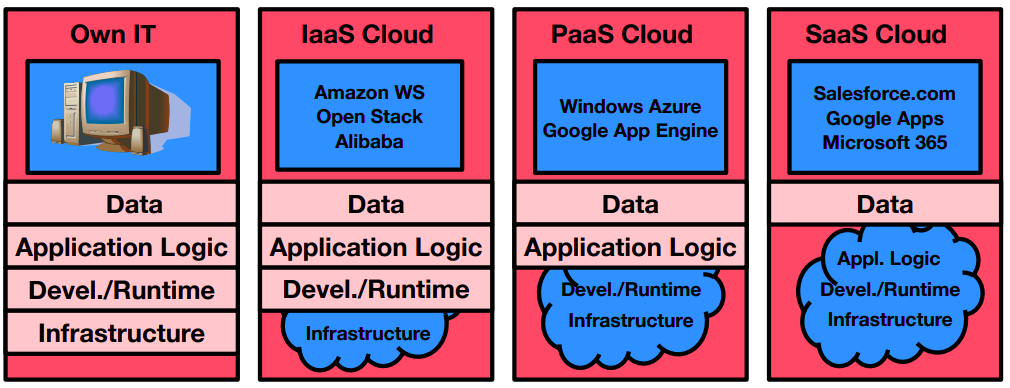
\includegraphics[width=\textwidth]{servicemodels.png}
	%\caption{Comparison over the service models}
\end{figure}
\begin{figure}[H]
	\centering
	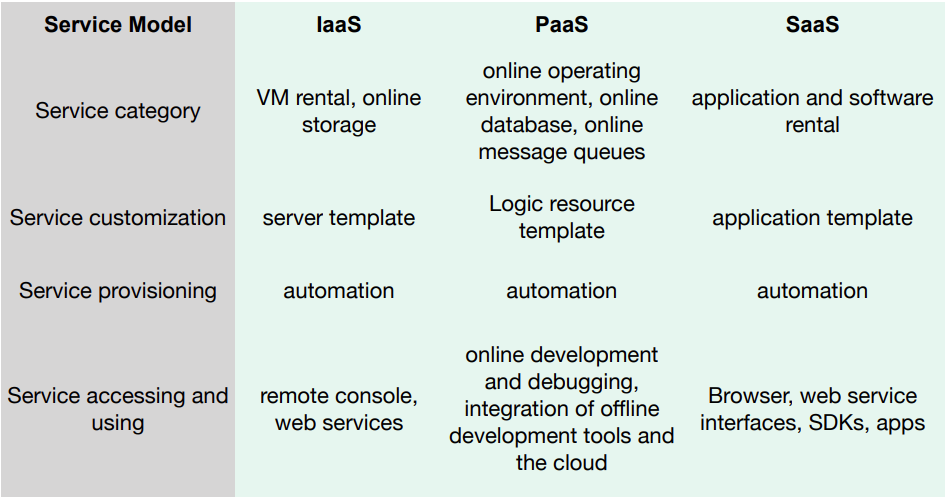
\includegraphics[width=0.8\textwidth]{servicemodel1.png}
	%\caption{Comparison over the service models}
\end{figure}\begin{figure}[H]
\centering
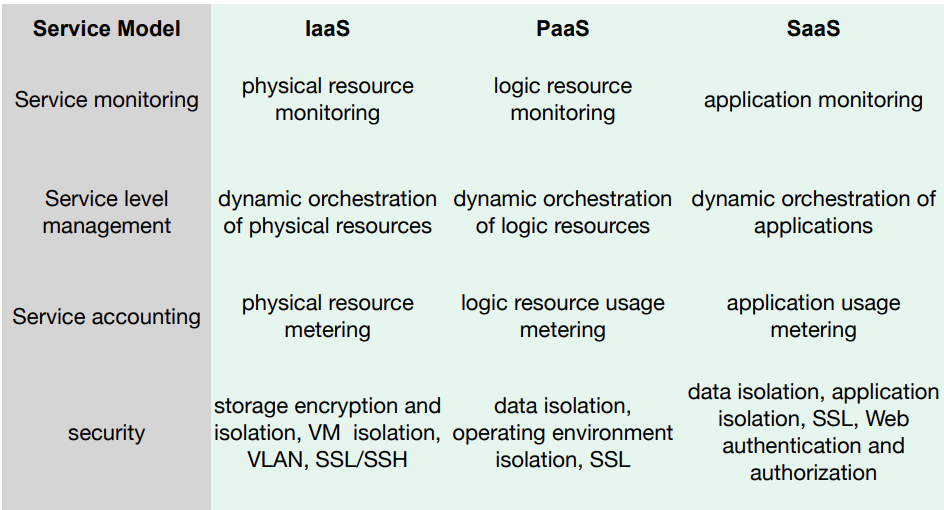
\includegraphics[width=0.8\textwidth]{servicemodel2.png}
%\caption{Comparison over the service models}
\end{figure}
\subsection{4 Deployment Models: Private, Community, Public, Hybrid}
\begin{itemize}
	\item Private Cloud:
	\begin{itemize}
		\item service offered \textbf{via private network} for \textbf{single client}.
	\end{itemize}
	\item Community Cloud:
	\begin{itemize}
		\item service offered to \textbf{a specific group of clients}.
	\end{itemize}
	\item Public Cloud:
	\begin{itemize}
		\item service offered \textbf{over Internet via Web-application} or third-party provider for \textbf{everyone}.
	\end{itemize}
	\item Hybrid Cloud: combination of public and private cloud.
\end{itemize}

\subsection{5 Essential Characteristics}
\begin{itemize}
	\item \textbf{on-demand self-service}: 
	\begin{itemize}
		\item able to \textbf{provision computing capabilities} unilaterally(no interaction required with provider).
	\end{itemize}
	
	\item \textbf{broad network access}: 
	\begin{itemize}
		\item capabilities can be available and accessed through by \textbf{diversely thin or thick client platforms} (mobile, tablets, cable, etc.)
	\end{itemize}
	
	\item \textbf{resource pooling}: 
	\begin{itemize}
		\item \textbf{multi-tenant model} is used, multiple customers shares the computing capabilities at the same time, according to their self-customized demand. Specification of resource location can be possible at higher abstraction level.
	\end{itemize}
	 
	\item \textbf{rapid elasticity}: 
	\begin{itemize}
		\item computing capabilities can be \textbf{elastically provisioned and released} in any quantity at any time. The process can be automated or scaled according to dynamic demand.
	\end{itemize}
	\item \textbf{measured service}: 
	\begin{itemize}
		\item automatically control and optimize resource use by \textbf{leveraging a metering capability}. Resource usage can be monitored, controlled and reported.
	\end{itemize}
\end{itemize}


\subsection{Pros \& Cons of Clouds}
\begin{itemize}
	\item Advantages:

\begin{itemize}
	\item scalability, elasticity
	\item rapid deployment
	\item no capital investment for physical resources
	\item outsourcing of infrastructure management
	\item limited access to on-premise servers
	\item fault tolerance: multiple servers have data replicas, if one node fails, other nodes will replace.
	\item collaboration
\end{itemize}
	\item Disadvantages:
	\begin{itemize}
		\item no control over security, based on ''trust''.
		\item no control over hardware/infrastructure
		\item vendor lockin: service is not standardized, not compatible to other vendors.
		\item cost on monthly fees: if demand for same computational power is constant, fee may be higher than building own hardware. Only recommendable for dynamic demand.
		\item breaking SLAs: your performance may be influenced by other tenants(multi-tenant model).
	\end{itemize}
\end{itemize}